% Kapitel 3 mit den entsprechenden Unterkapiteln
% Die Unterkapitel können auch in separaten Dateien stehen,
% die dann mit dem \include-Befehl eingebunden werden.
%-------------------------------------------------------------------------------
\chapter{Implementierungsentwurf}

In diesem Kapitel werden die Implementierungsdetails für die Umsetzung des
Grobentwurfs vorgestellt. Gegenüber letzterem werden neben den Schnittstellen
auch die Implementierungen spezifiziert. Die Abbildungen zeigen die 
Klassenhierachie in den jeweiligen Paketen. Aus Gründen der Übersichtlichkeit
wird in den Implementierungen auf die Auflistung der Operationen der Schnittstellen
verzichtet.

\begin{figure}[!h]
	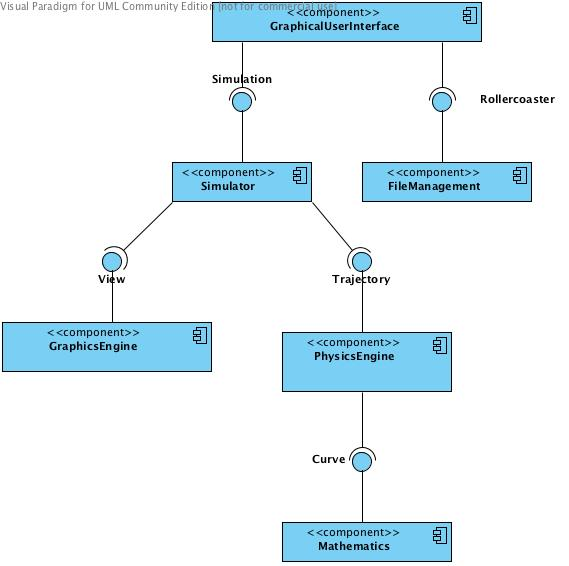
\includegraphics[width=0.8\linewidth]{bilder/components.jpg}
\caption{Komponentendiagramm}
\end{figure}


\section{Gesamtsystem}
Fügen Sie hier bitte das Komponentendiagramm aus dem Grobentwurf ein und
erläutern Sie kurz die Funktionen der Komponenten.
%%%%%%%%%%%%%%%%%%%%%%%%%%%%%%%%%%%%%%%%%%%%%%%%%%%%%%%%%%%%
\section{Implementierung von Komponente
         <ID aus Grobentwurf>: <Komponentenname>:}

Beschreiben Sie hier bitte die Implementierung der Komponente. Erläutern Sie
bitte dabei, welche Entwurfsmuster und Bibliotheken Sie verwenden. Die
Implementierung wird dabei durch Klassendiagramme dokumentiert.

\subsection{Paketdiagramm}
\subsection{Erläuterung}

Die verwendeten Attribute, Aufgaben und Kommunikationspartner sind für jede
Klasse kurz zu erläutern. Die ankommenden Nachrichten beziehen sich dabei auf
die Sequenzdiagramme der Feinanalyse im Grobentwurf und stellen meist
aufzurufende Methoden der Klasse dar.  Reine get- / set-Methoden oder
Bibliotheksfunktionen brauchen nicht aufgeführt zu werden.


%%%%%%%%%%%%%%%%%%%%%%%%%%%%%%%%%%%%%%%%%%%%%%%%%%%%%%%%%%%%
\subsubsection{Implementierung von Komponente
         xx: Graphics3D:}

\textbf {Dieser Bereich ist noch nicht entgültig fertig,bedarf einer Überarbeitung und steht zur Diskussion!}

\begin{figure}
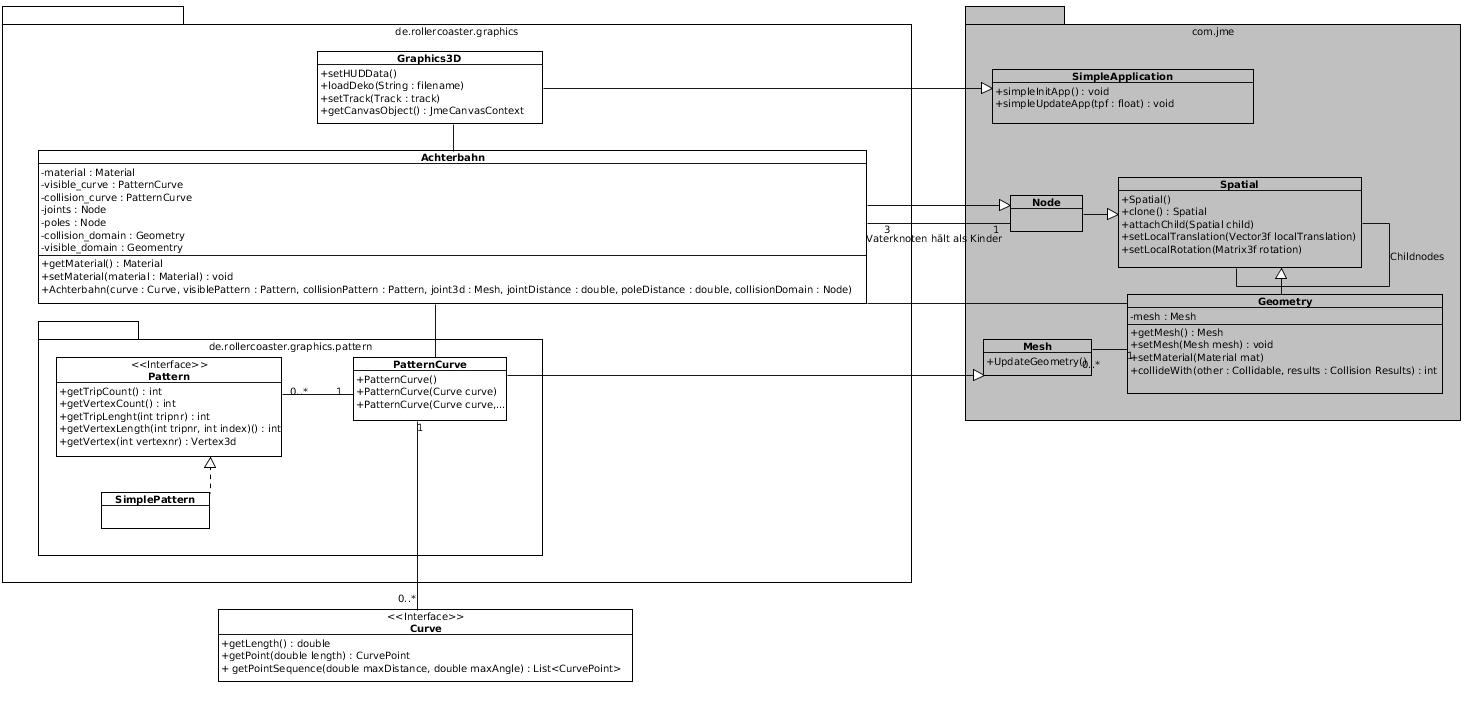
\includegraphics[width=\linewidth]{bilder/klassendiagramm_004}
\caption{Klassendiagrammname}
\end{figure}

Die JMonkeyEngine stellt eine Scenegraphenstruktur über Spatial zur Verfügung die hier kurz skizziert wird. Die Subklassen Geometry als Meshcontainer und Node als Strukturelement werden von unserer Hauptklasse Achterbahn 
zur Speicherung und Ordnung der Geometrieelemente verwendet. PatternCurve ist eine Klasse die ein Pattern entlang einer Curve extrudiert.

\begin{figure}
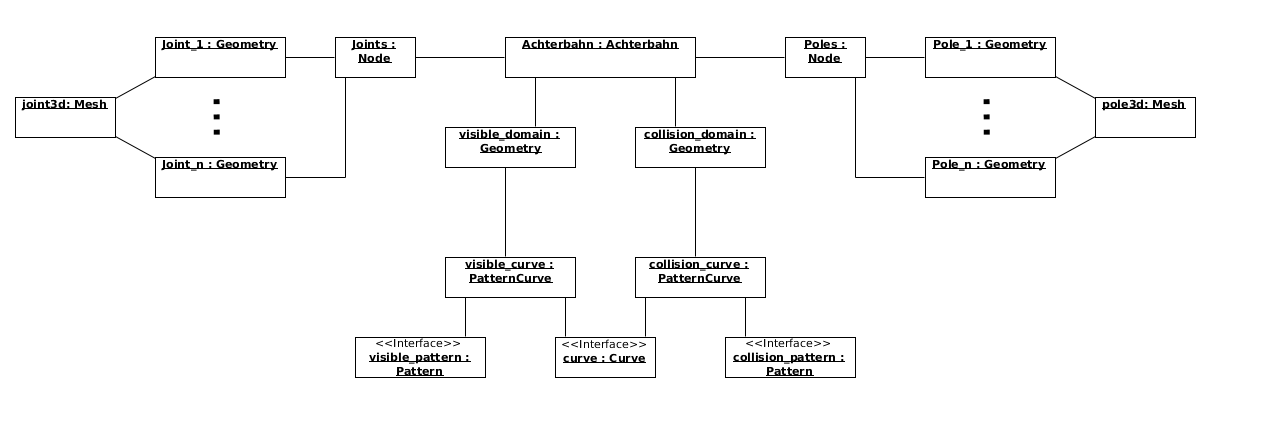
\includegraphics[width=\linewidth]{bilder/objektdiagramm_004}
\caption{Objektidagrammname}
\end{figure}

Im wesentlichen hält die Achterbahn 4 Knoten. Unter joints hängen alle n Geomentrien die auf die gleiche Mesh zeigen und die Verbindungsstücke der Bahn erzeugen. Das Konzept erlaubt, dass in jedem Geometry eigene Rotation und 
Translation gesetzt werden, sodass die Mesh an unterschiedlichen Orten im 3D-Raum gezeichnet wird, ohne jedoch die Mesh im Speicher vollständig kopieren zu müssen. Poles enthält die Stützpfeiler der Bahn und ist analog strukturiert.
Die Schienen werden in der visible\_domain durch eine PatternCurve erzeugt. In der collision\_domain liegt eine zweite PatternCurve, die ein BoundingVolume um die Bahn definiert um Kollisionen mit bereits geladener oder neu zu ladener
Dekoration zu erkennen. Dieses BoundingVolume wird außerdem dazu verwendet die Stützpfeiler zu generieren, ohne dass diese in durch die Bahn ragen.



\subsection{Paketdiagramm}
\subsection{Erläuterung}

Die verwendeten Attribute, Aufgaben und Kommunikationspartner sind für jede
Klasse kurz zu erläutern. Die ankommenden Nachrichten beziehen sich dabei auf
die Sequenzdiagramme der Feinanalyse im Grobentwurf und stellen meist
aufzurufende Methoden der Klasse dar.  Reine get- / set-Methoden oder
Bibliotheksfunktionen brauchen nicht aufgeführt zu werden.

%%%%%%%%%%%%%%%%%%%%%%%%%%%%%%%%%%%%%%%%%%%%%%%%%%%%%%%%%%%%
\section{Implementierung von Komponente
         <ID aus Grobentwurf>: Data:}

Beschreibung folgt

\subsection{Paketdiagramm}

\begin{figure}
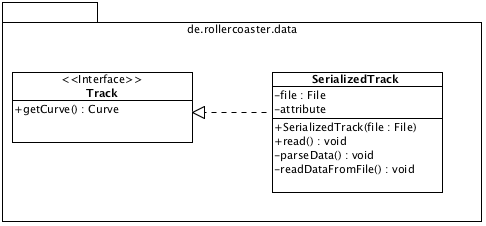
\includegraphics[width=\linewidth]{bilder/Data}
\caption{Daten}
\end{figure}

\subsection{Erläuterung}

Erläuterung folgt

%%%%%%%%%%%%%%%%%%%%%%%%%%%%%%%%%%%%%%%%%%%%%%%%%%%%%%%%%%%%
\section{Implementierung von Komponente
         <ID aus Grobentwurf>: Mathematics:}

Beschreibung folgt

\subsection{Paketdiagramm}

\begin{figure}
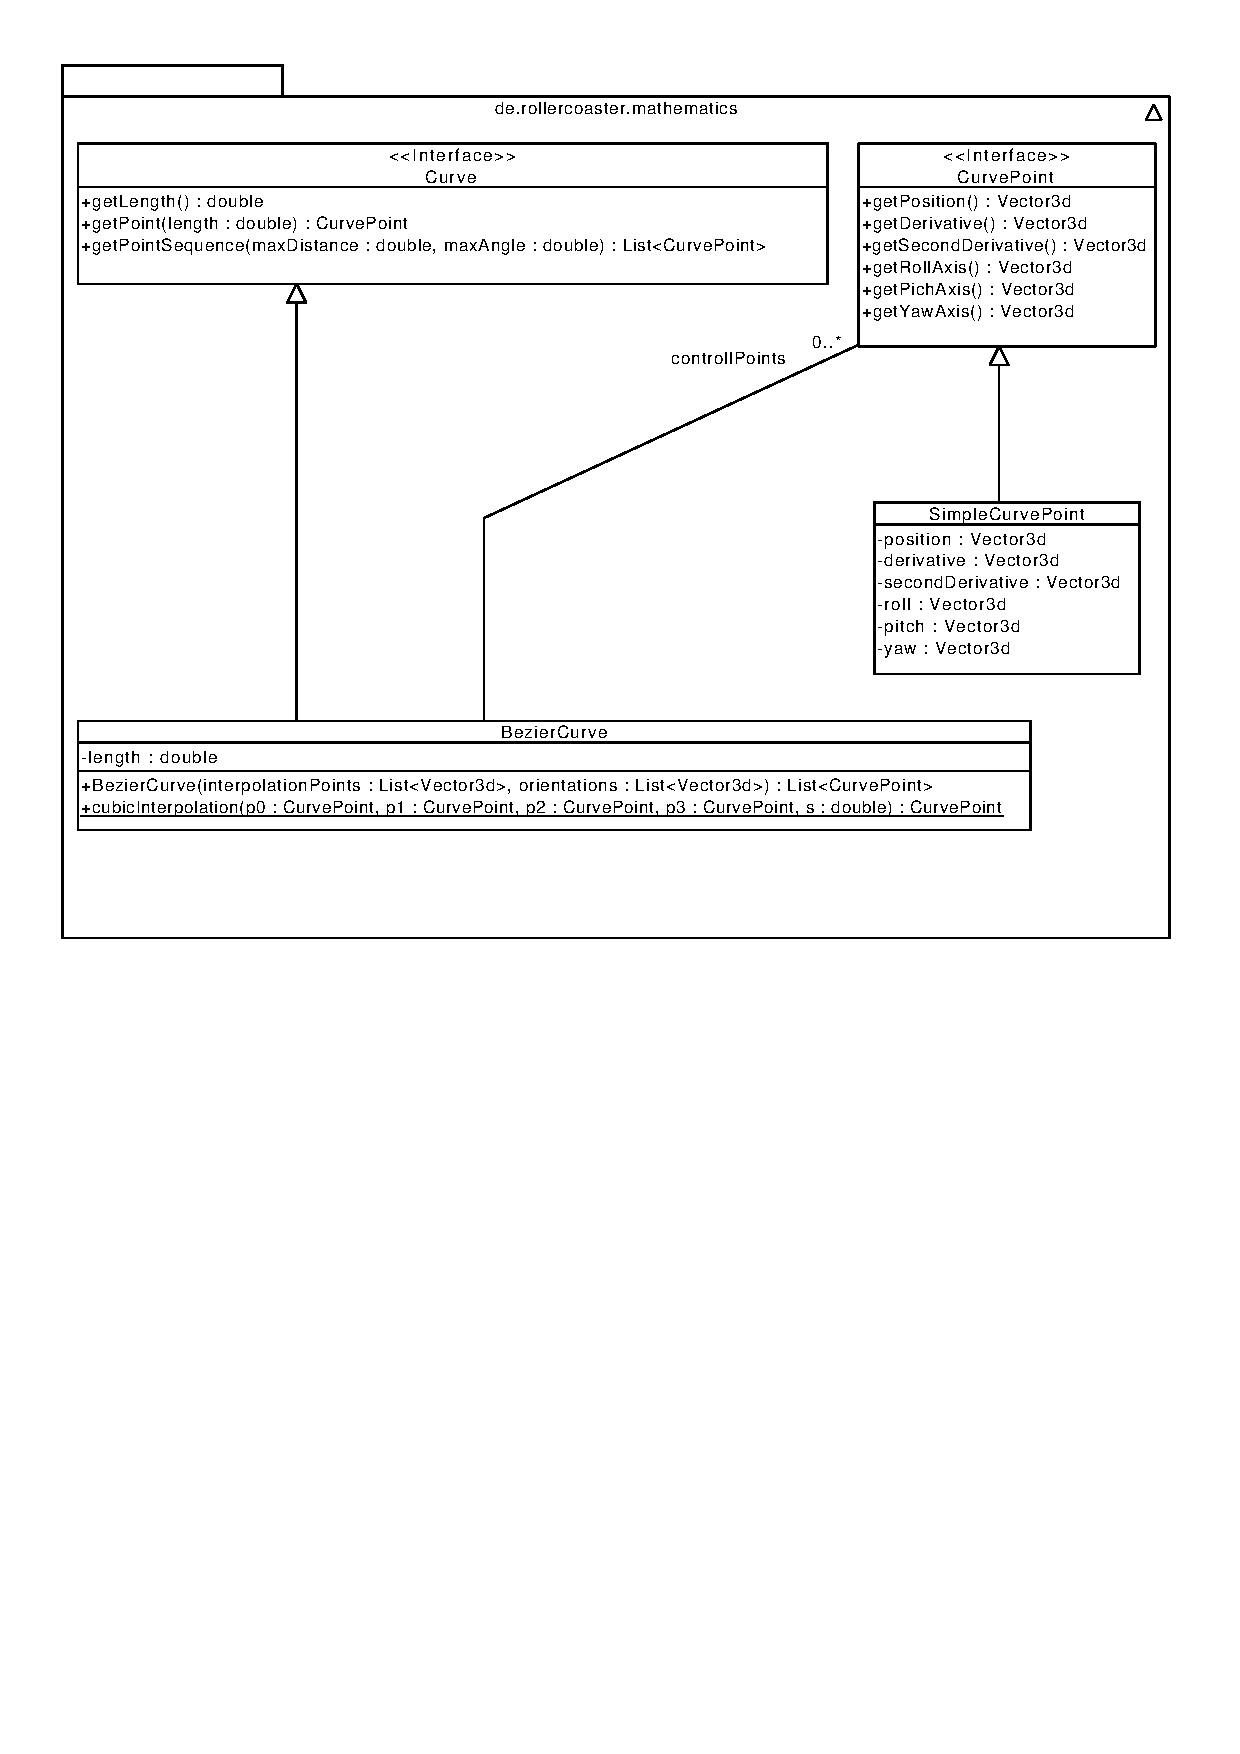
\includegraphics[width=\linewidth]{bilder/Mathematics}
\caption{Mathe}
\end{figure}
\begin{figure}
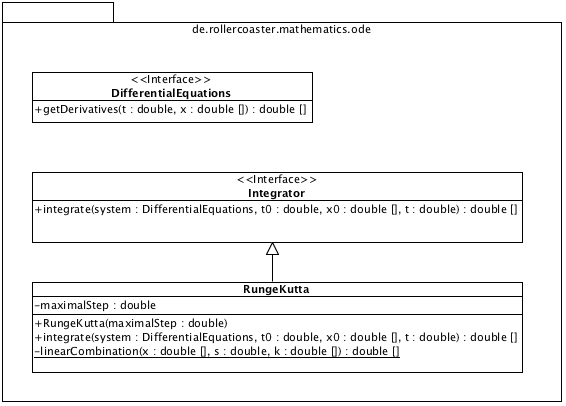
\includegraphics[width=\linewidth]{bilder/Mathematics_ODE}
\caption{Mathe}
\end{figure}

\subsection{Erläuterung}

Erläuterung folgt

%%%%%%%%%%%%%%%%%%%%%%%%%%%%%%%%%%%%%%%%%%%%%%%%%%%%%%%%%%%%
\section{Implementierung von Komponente
         <ID aus Grobentwurf>: Physics:}

Beschreibung folgt

\subsection{Paketdiagramm}
\begin{figure}
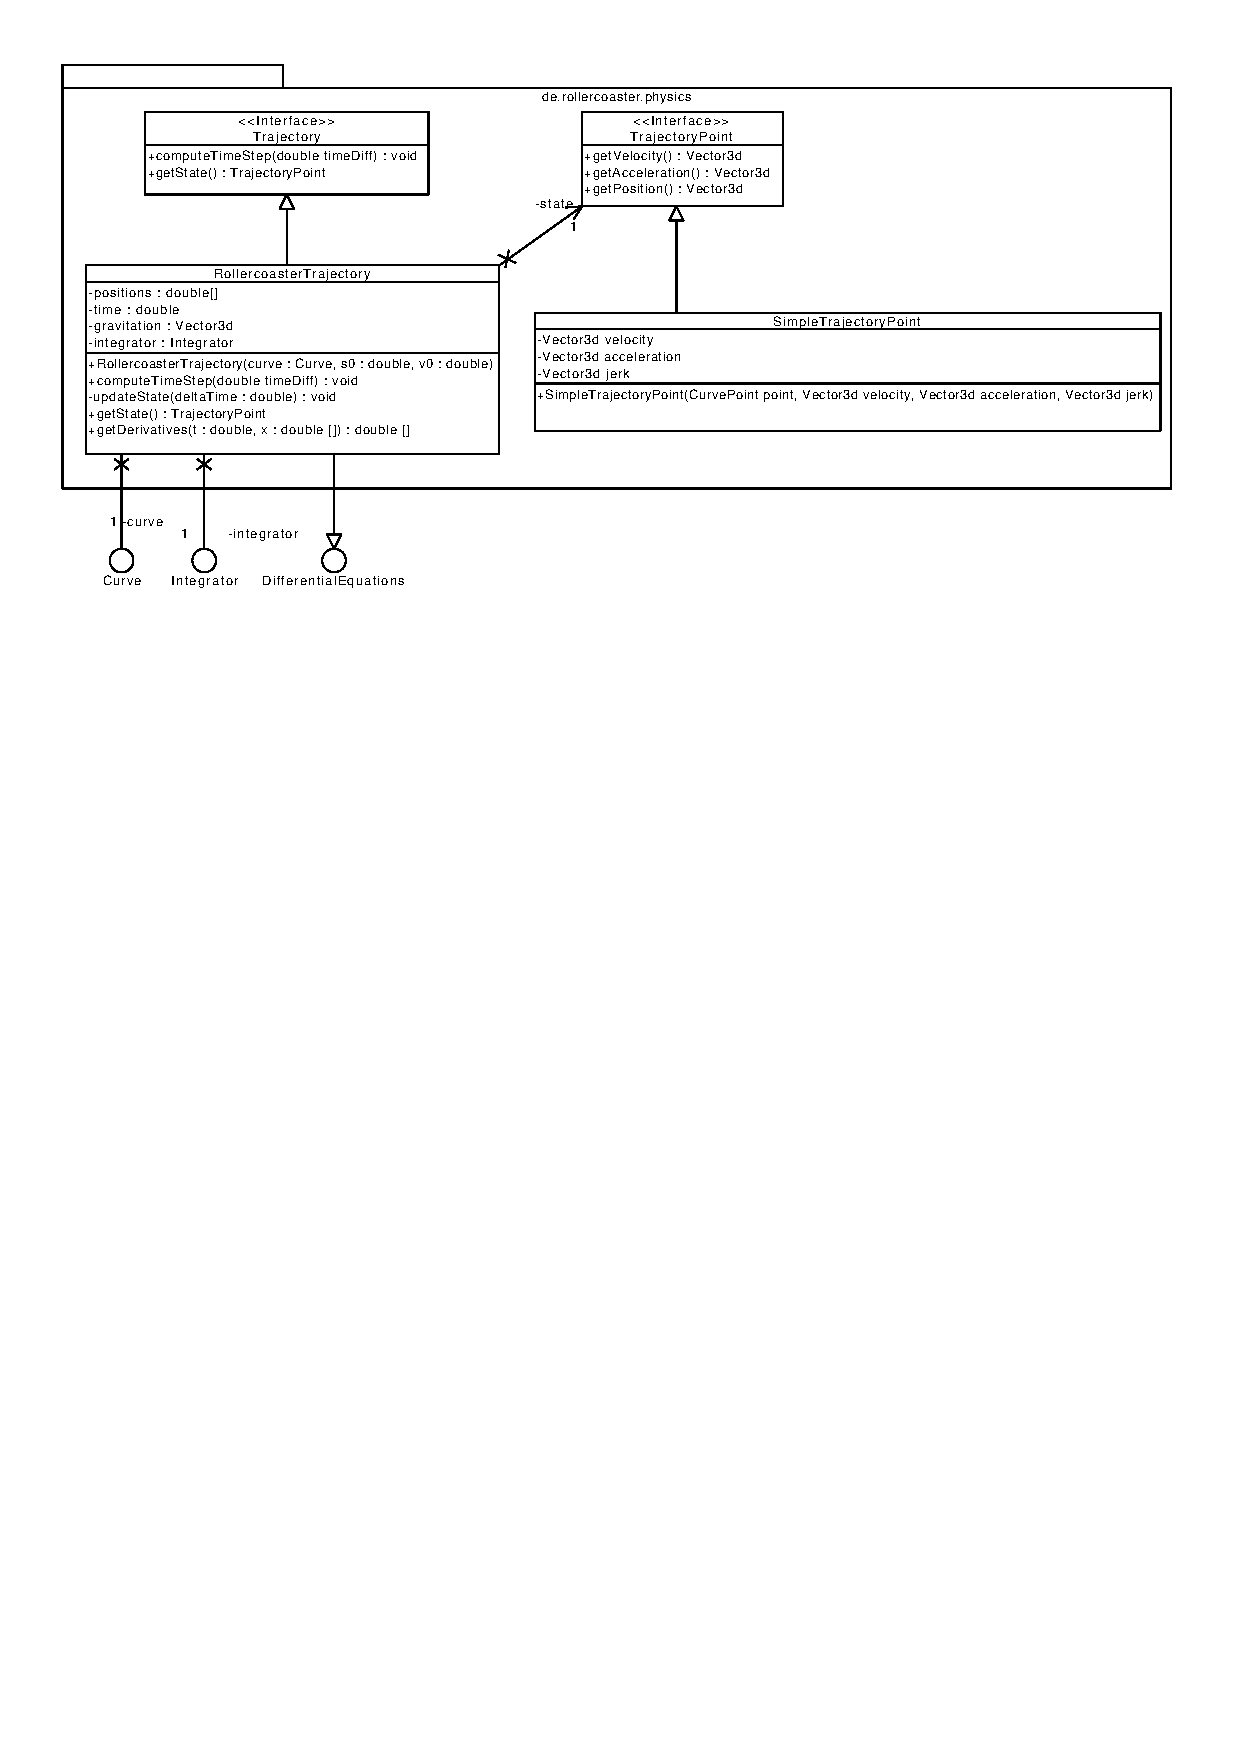
\includegraphics[width=\linewidth]{bilder/Physics}
\caption{Physik}
\end{figure}

\subsection{Erläuterung}

Erläuterung folgt


%%%%%%%%%%%%%%%%%%%%%%%%%%%%%%%%%%%%%%%%%%%%%%%%%%%%%%%%%%%%
\section{Implementierung von Komponente
         <ID aus Grobentwurf>: Simulation:}

Beschreibung folgt

\subsection{Paketdiagramm}
\begin{figure}
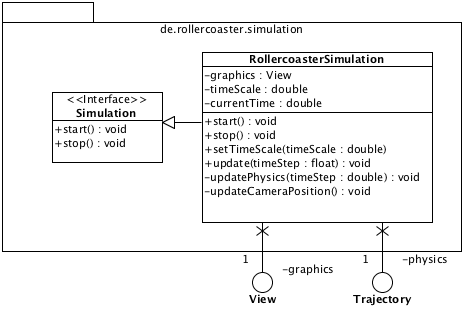
\includegraphics[width=\linewidth]{bilder/Simulation}
\caption{Simulation}
\end{figure}

\subsection{Erläuterung}

Erläuterung folgt
